% !TeX program = xelatex
\ifdefined\BookMaster\else
\documentclass[11pt,oneside]{article}
% !TeX program = xelatex
\usepackage[b5paper,left=22mm,right=22mm,top=20mm,bottom=22mm,footskip=11mm]{geometry}
\usepackage{fontspec}
\setmainfont{TeX Gyre Termes}
\setsansfont{TeX Gyre Heros}
\usepackage{amsmath,amssymb,mathtools,amsthm}
\renewcommand{\cdots}{\mathinner{\cdotp\cdotp\cdotp}}
\usepackage{graphicx,adjustbox,array,booktabs,longtable,multirow,enumitem,changepage,needspace}
\usepackage[table]{xcolor}
\usepackage{fancyhdr}
\raggedbottom
\interfootnotelinepenalty=10000
\newcommand{\BookFootnote}[2]{\begingroup\renewcommand{\thefootnote}{\fnsymbol{footnote}}\footnote[#1]{#2}\endgroup}
\newcommand{\BookFootnoteMark}[1]{\begingroup\renewcommand{\thefootnote}{\fnsymbol{footnote}}\footnotemark[#1]\endgroup}
\newcommand{\BookFootnoteText}[2]{\begingroup\renewcommand{\thefootnote}{\fnsymbol{footnote}}\footnotetext[#1]{#2}\endgroup}
\newenvironment{BookFloat}[1]{\par\addvspace{.6\baselineskip}\noindent\def\BookFloatID{#1}\begin{minipage}{\linewidth}\phantomsection\label{bookfloat:#1:start}}{\phantomsection\label{bookfloat:\BookFloatID:end}\end{minipage}\par\addvspace{.6\baselineskip}}

\usepackage[unicode,hidelinks]{hyperref}
\pagestyle{fancy}
\fancyhf{}
\newcommand{\BookFooter}{}
\fancyfoot[L]{\parbox[b]{\dimexpr\textwidth-15mm}{\footnotesize\BookFooter}}
\fancyfoot[R]{\footnotesize\thepage}
\renewcommand{\headrulewidth}{0pt}
\renewcommand{\footrulewidth}{0pt}
\setlength{\parindent}{0pt}
\setlength{\parskip}{0.2em}
\setlength{\emergencystretch}{3em}
\setlist{nosep,leftmargin=1.7em,labelsep=.65em}
\newif\ifBookNarrative
\BookNarrativetrue
\newenvironment{BookBody}{\setlength{\parindent}{0pt}}{}
\newcommand{\BookStatement}[1]{\par\addvspace{.6\baselineskip}\noindent #1\enspace\ignorespaces}
\newcommand{\BookLabel}[1]{\par\addvspace{.6\baselineskip}\needspace{3\baselineskip}\noindent\textbf{#1}\quad\ignorespaces}
\newcommand{\BookHeading}[1]{\par\addvspace{\baselineskip}\needspace{4\baselineskip}\noindent{\large\bfseries #1}\par\medskip}
\newcommand{\BookSubheading}[1]{\par\addvspace{.7\baselineskip}\needspace{3\baselineskip}\noindent{\bfseries #1}\par\smallskip}
\newcommand{\BookTextHeading}[1]{\par\addvspace{.7\baselineskip}\needspace{3\baselineskip}\noindent #1\par\smallskip}
\newcommand{\BookSectionTitle}[2]{\par\addvspace{1.2\baselineskip}\needspace{5\baselineskip}\noindent\colorbox{gray!25}{\sffamily\bfseries\small SECTION #1}\quad{\large\bfseries #2}\par\medskip}
\newcommand{\BookExerciseTitle}[1]{\par\addvspace{\baselineskip}\needspace{4\baselineskip}\noindent{\color{gray}\rule{1.5mm}{1.5mm}}\enspace{\large\bfseries Exercises #1}\par\medskip}
\newcommand{\BookBullet}[1]{\begin{list}{\textbullet}{\setlength{\leftmargin}{1.7em}\setlength{\labelwidth}{1em}\setlength{\labelsep}{.7em}\setlength{\topsep}{0pt}\setlength{\parsep}{0pt}\setlength{\itemsep}{0pt}}\item #1\end{list}}
\newcommand{\BookExercise}[2]{\begin{list}{\textbf{#1}}{\setlength{\leftmargin}{2.2em}\setlength{\labelwidth}{1.5em}\setlength{\labelsep}{.7em}\setlength{\topsep}{.15em}\setlength{\parsep}{0pt}\setlength{\itemsep}{0pt}}\item #2\end{list}}
\newcommand{\BookEnd}[1]{\unskip\nobreak\hfill\ensuremath{#1}}
\newcommand{\BookSource}[2]{\phantomsection\label{sourcepage:#1}} % Source-page anchors, retained through reflow.
\usepackage{multicol}
\usepackage{tikz}
\newcommand{\BookPartEntry}[2]{\par\noindent\makebox[17mm][l]{\bfseries Section #1}#2\par}
\newcommand{\BookPartTitle}[3]{\par\bigskip\noindent\begin{tikzpicture}\node[anchor=north west,inner sep=0pt,outer sep=0pt] (bookpart) at (0,0) {\begin{minipage}{\dimexpr\linewidth-.5pt}\hspace*{26mm}\begin{minipage}[t]{\dimexpr\linewidth-26mm}\begin{adjustbox}{max width=\linewidth}{\fontsize{20}{24}\selectfont\bfseries #2}\end{adjustbox}\par\vspace{6mm}\hrule\vspace{6mm}{\sffamily\footnotesize\setlength{\parskip}{.3em}#3}\vspace{3mm}\end{minipage}\end{minipage}};\path[shade,top color=gray!60,bottom color=white] (0,0) rectangle ([xshift=24mm]bookpart.south west);\node[anchor=north,font=\sffamily\bfseries\small] at (12mm,-2mm) {PART};\node[anchor=north,font=\sffamily\bfseries\Huge] at (12mm,-7mm) {#1};\end{tikzpicture}\par\bigskip}
\newsavebox{\BookMathBox}
\makeatletter
\newcommand{\BookInline}[1]{\leavevmode\hskip0pt\relax\begingroup\in@{\begin}{#1}\ifin@\sbox{\BookMathBox}{\(#1\)}\ifdim\wd\BookMathBox>\dimexpr\linewidth-1em\relax\resizebox{\dimexpr\linewidth-1em\relax}{!}{\usebox{\BookMathBox}}\else\(#1\)\fi\else\in@{\left}{#1}\ifin@\sbox{\BookMathBox}{\(#1\)}\ifdim\wd\BookMathBox>\dimexpr\linewidth-1em\relax\resizebox{\dimexpr\linewidth-1em\relax}{!}{\usebox{\BookMathBox}}\else\(#1\)\fi\else\(#1\)\fi\fi\endgroup\hskip0pt\relax}
\makeatother
\DeclareMathOperator{\Aut}{Aut}
\DeclareMathOperator{\End}{End}
\DeclareMathOperator{\Hom}{Hom}
\DeclareMathOperator{\GF}{GF}
\DeclareMathOperator{\irr}{irr}
\DeclareMathOperator{\lt}{lt}
\DeclareMathOperator{\lp}{lp}
\providecommand{\textcircled}[1]{\textnormal{(#1)}}

\begin{document}
\fi
\renewcommand{\BookFooter}{Section 26 the Field of Quotients of an Integral Domain}
\pdfbookmark[0]{Section 26 the Field of Quotients of an Integral Domain}{26_the_field_of_quotients_of_an_integral_domain}
\ifdefined\BookMaster\else\setcounter{page}{211}\fi
% Source PDF page 228; original printed page 211
\BookSource{228}{211}
\BookPartTitle{VI}{Constructing Rings and Fields}{\BookPartEntry{26}{the Field of Quotients of an Integral Domain}
\BookPartEntry{27}{Rings of Polynomials}
\BookPartEntry{28}{Factorization of Polynomials over a Field}
\BookPartEntry{29}{Algebraic Coding Theory}
\BookPartEntry{30}{Homomorphisms and Factor Rings}
\BookPartEntry{31}{Prime and Maximal Ideals}
\BookPartEntry{32}{Noncommutative Examples}}

\BookNarrativetrue

\begin{BookBody}

\BookSectionTitle{26}{the Field of Quotients of an Integral Domain}

\noindent Let \BookInline{L} be a field and \BookInline{D} a subring of \BookInline{L} that contains the unity. The ring \BookInline{D} is an integral domain since it has no zero divisors. Also \BookInline{F,\allowbreak } the set of all quotients of the form \BookInline{\frac{a}{b}} with \BookInline{a} and \BookInline{b\neq 0} both in \BookInline{D,\allowbreak } forms a subfield of \BookInline{L.} The field \BookInline{F} is called a \BookInline{\text{fi}eld} \textit{of quotients of} \textit{the integral domain} \BookInline{D.}

\BookLabel{26.1 Example} Let \BookInline{L= \mathbb{R}.} If \BookInline{D= \mathbb{Z},\allowbreak } then

\begin{center}\begin{adjustbox}{max width=\linewidth}\BookInline{\displaystyle F = \left\{ \frac{a}{b} \; \middle| \; a,\allowbreak  b \in \mathbb{Z},\allowbreak  b \neq 0 \right\} = \mathbb{Q}}\end{adjustbox}\end{center}

\noindent which is a field.

If \BookInline{D= \{x+ y\sqrt{2}\mid x,\allowbreak y\in \mathbb{Z}\},\allowbreak } then

\begin{center}\begin{adjustbox}{max width=\linewidth}\BookInline{\displaystyle F = \left\{ \frac{a}{b} \left| a,\allowbreak  b \in D,\allowbreak  b \neq 0 \right\} = \left\{ \frac{x + y\sqrt{2}}{z + w\sqrt{2}} \right| x,\allowbreak  y,\allowbreak  z,\allowbreak  w \in \mathbb{Z},\allowbreak  z + w\sqrt{2} \neq 0 \right\}.}\end{adjustbox}\end{center}

\noindent By rationalizing the denominator we see that

\begin{center}\begin{adjustbox}{max width=\linewidth}\BookInline{\displaystyle F = \left\{ r + s { \sqrt { 2 } }   |   r ,\allowbreak  s \in \mathbb { Q } \right\}}\end{adjustbox}\end{center}

\noindent which is a field by Exercise 12 in Section 22. \BookEnd{\blacktriangle}

In this section, we start with an integral domain \BookInline{D} and construct a field \BookInline{F.} We then show that \BookInline{D} is isomorphic with a subring \BookInline{D^{\prime }} of \BookInline{F} and that \BookInline{F} consists of all quotients \BookInline{\frac{a}{b}} with \BookInline{a,\allowbreak b\in D^{\prime },\allowbreak b\neq 0.} Thus we can think of any integral domain as being a subring of a field and every element of the field is the quotient of elements from the integral domain.

\BookTextHeading{\textbf{The Construction}  }

\noindent Let \BookInline{D} be an integral domain that we desire to enlarge to a field of quotients \BookInline{F.} A coarse outline of the steps we take is as follows:

\BookExercise{1.}{Define what the elements of \BookInline{F} are to be.}

\BookExercise{2.}{Define the binary operations of addition and multiplication on \BookInline{F.}}

\end{BookBody}

% Source PDF page 229; original printed page 212
\BookSource{229}{212}
\BookNarrativetrue

\begin{BookBody}

\BookExercise{3.}{Check all the field axioms to show that \BookInline{F} is a field under these operations.}

\BookExercise{4.}{Show that \BookInline{F} can be viewed as containing \BookInline{D} as an integral subdomain.}

\noindent Steps 1, 2, and 4 are very interesting, and Step 3 is largely a mechanical chore. We proceed with the construction.

\textbf{Step 1} Let \BookInline{D} be a given integral domain, and form the Cartesian product

\begin{center}\begin{adjustbox}{max width=\linewidth}\BookInline{\displaystyle D\times D= \{(a,\allowbreak b)\mid a,\allowbreak b\in D\}}\end{adjustbox}\end{center}

\noindent We are going to think of an ordered pair \BookInline{(a,\allowbreak b)} as representing a\textit{ formal quotient} \BookInline{a/b,\allowbreak } that is, if \BookInline{D= \mathbb{Z},\allowbreak } the pair (2, 3) will eventually represent the number \BookInline{\frac{2}{3}} for us. The pair (2, 0) represents no element of \BookInline{\mathbb{Q}} and suggests that we cut the set \BookInline{D\times D} down a bit. Let \BookInline{S} be the subset of \BookInline{D\times D} given by

\begin{center}\begin{adjustbox}{max width=\linewidth}\BookInline{\displaystyle S= \{(a,\allowbreak b)\mid a,\allowbreak b\in D,\allowbreak b\neq  0\}.}\end{adjustbox}\end{center}

\noindent Now \BookInline{S} is still not going to be our field as is indicated by the fact that, with \BookInline{D= \mathbb{Z},\allowbreak } \textit{different} pairs of integers such as (2, 3) and (4, 6) can represent the\textit{ same} rational number. We next define when two elements of \BookInline{S} will eventually represent the same element of \BookInline{F,\allowbreak } or, as we shall say, when two elements of \BookInline{S} are\textit{ equivalent}.

\BookLabel{26.2 Definition} Two elements \BookInline{(a,\allowbreak b)} and \BookInline{(c,\allowbreak d)} in \BookInline{S} are\textbf{ equivalent,} denoted by \BookInline{(a,\allowbreak b)\sim (c,\allowbreak d),\allowbreak } if and only if \BookInline{ad= bc.}\BookEnd{\blacksquare}

Observe that this definition is reasonable, since the criterion for \BookInline{(a,\allowbreak b)\sim (c,\allowbreak d)} is an equation \BookInline{ad= bc} involving elements in \BookInline{D} and concerning the known multiplication in \BookInline{D.} Note also that for \BookInline{D= \mathbb{Z},\allowbreak } the criterion gives us our usual definition of\textit{ equality} of \BookInline{\frac{a}{b}} with \BookInline{\frac { c } { d },\allowbreak } for example, \BookInline{{ \textstyle { \frac { 2 } { 3 } } = { \frac { 4 } { 6 } } }} since \BookInline{(2)(6)= (3)(4).} The rational number that we usually denote by \BookInline{\frac{2}{3}} can be thought of as the collection of\textit{ all} quotients of integers that reduce to, or are equivalent to, 23.

\BookLabel{26.3 Lemma} The relation \BookInline{\sim } between elements of the set \BookInline{S} as just described is an equivalence relation.

\BookLabel{\textit{Proof}} We must check the three properties of an equivalence relation.

\textbf{Reflexive} \BookInline{(a,\allowbreak b)\sim (a,\allowbreak b)} since \BookInline{ab= ba,\allowbreak } for multiplication in \BookInline{D} is commutative.

\textbf{Symmetric} If \BookInline{(a,\allowbreak b)\sim (c,\allowbreak d),\allowbreak } then \BookInline{ad= bc.} Since multiplication in \BookInline{D} is commutative, we deduce that \BookInline{cb= da,\allowbreak } and consequently \BookInline{(c,\allowbreak d)\sim (a,\allowbreak b).}

\textbf{Transitive} If \BookInline{(a,\allowbreak b)\sim (c,\allowbreak d)} and \BookInline{(c,\allowbreak d)\sim (r,\allowbreak s),\allowbreak } then \BookInline{ad= bc} and \BookInline{cs= dr.} Using these relations and the fact that multiplication in \BookInline{D} is commutative, we have

\begin{center}\begin{adjustbox}{max width=\linewidth}\BookInline{\displaystyle asd= sad= sbc= bcs= bdr= brd.}\end{adjustbox}\end{center}

Now \BookInline{d\neq 0,\allowbreak } and \BookInline{D} is an integral domain, so cancellation is valid; this is a crucial step in the argument. Hence from \BookInline{asd= brd} we obtain\textit{ as} \BookInline{= br,\allowbreak } so that \BookInline{(a,\allowbreak b)\sim (r,\allowbreak s).}\BookEnd{\blacklozenge}

We now know, in view of Theorem 0.22, that \BookInline{\sim } gives a partition of \BookInline{S} into equivalence classes. To avoid long bars over extended expressions, we shall let \BookInline{[(a,\allowbreak b)],\allowbreak } rather than \BookInline{(a,\allowbreak b),\allowbreak } be the equivalence class of \BookInline{(a,\allowbreak b)} in \BookInline{S} under the relation \BookInline{\sim.} We now finish Step 1 by defining \BookInline{F} to be the set of all equivalence classes \BookInline{[(a,\allowbreak b)]} for \BookInline{(a,\allowbreak b)\in S.}

\textbf{Step 2} The next lemma serves to define addition and multiplication in \BookInline{F.} Observe that if \BookInline{D= \mathbb{Z}} and \BookInline{[(a,\allowbreak b)]} is viewed as \BookInline{(a/b)\in \mathbb{Q},\allowbreak } these definitions applied to \BookInline{\mathbb{Q}} give the usual operations.

\end{BookBody}

% Source PDF page 230; original printed page 213
\BookSource{230}{213}
\BookNarrativetrue

\begin{BookBody}

\BookLabel{26.4 Lemma} For \BookInline{[(a,\allowbreak b)]} and \BookInline{[(c,\allowbreak d)]} in \BookInline{F,\allowbreak } the equations

\begin{center}\begin{adjustbox}{max width=\linewidth}\BookInline{\displaystyle [(a,\allowbreak b)]+ [(c,\allowbreak d)]= [(ad+ bc,\allowbreak bd)]}\end{adjustbox}\end{center}

\noindent and

\begin{center}\begin{adjustbox}{max width=\linewidth}\BookInline{\displaystyle [(a,\allowbreak b)][(c,\allowbreak d)]= [(ac,\allowbreak bd)]}\end{adjustbox}\end{center}

\noindent give well-defined operations of addition and multiplication on \BookInline{F.}

\BookLabel{\textit{Proof}} Observe first that if \BookInline{[(a,\allowbreak b)]} and \BookInline{[(c,\allowbreak d)]} are in \BookInline{F,\allowbreak } then \BookInline{(a,\allowbreak b)} and \BookInline{(c,\allowbreak d)} are in \BookInline{S,\allowbreak } so \BookInline{b\neq 0} and \BookInline{d\neq 0.} Because \BookInline{D} is an integral domain\BookInline{,\allowbreak bd\neq 0,\allowbreak } so both \BookInline{(ad+ bc,\allowbreak bd)} and (\textit{ac}\BookInline{,\allowbreak bd)} are in \BookInline{S.(}Note the crucial use here of the fact that \BookInline{D} has no divisors of 0.) This shows that the right-hand sides of the defining equations are at least in \BookInline{F.}

It remains for us to show that these operations of addition and multiplication are well defined. That is, they were defined by means of representatives in \BookInline{S} of elements of \BookInline{F,\allowbreak } so we must show that if different representatives in \BookInline{S} are chosen, the same element of \BookInline{F} will result. To this end, suppose that \BookInline{(a_{1},\allowbreak b_{1})\in [(a,\allowbreak b)]} and \BookInline{(c_{1},\allowbreak d_{1})\in [(c,\allowbreak d)].} We must show that

\begin{center}\begin{adjustbox}{max width=\linewidth}\BookInline{\displaystyle (a_{1}d_{1}+ b_{1}c_{1},\allowbreak b_{1}d_{1})\in [(ad+ bc,\allowbreak bd)]}\end{adjustbox}\end{center}

\noindent and

\begin{center}\begin{adjustbox}{max width=\linewidth}\BookInline{\displaystyle (a_{1}c_{1},\allowbreak b_{1}d_{1})\in [(ac,\allowbreak bd)].}\end{adjustbox}\end{center}

\noindent Now \BookInline{(a_{1},\allowbreak b_{1})\in [(a,\allowbreak b)]} means that \BookInline{(a_{1},\allowbreak b_{1})\sim (a,\allowbreak b);} that is,

\begin{center}\begin{adjustbox}{max width=\linewidth}\BookInline{\displaystyle a_{1}b= b_{1}a.}\end{adjustbox}\end{center}

\noindent Similarly\BookInline{,\allowbreak (c_{1},\allowbreak d_{1})\in [(c,\allowbreak d)]} implies that

\begin{center}\begin{adjustbox}{max width=\linewidth}\BookInline{\displaystyle c_{1}d= d_{1}c.}\end{adjustbox}\end{center}

\noindent To get a “common denominator” (common second member) for the four pairs \BookInline{(a,\allowbreak b),\allowbreak } \BookInline{(a_{1},\allowbreak b_{1}),\allowbreak (c,\allowbreak d),\allowbreak } and \BookInline{(c_{1},\allowbreak d_{1}),\allowbreak } we multiply the first equation by \BookInline{d_{1}d} and the second equation by \BookInline{b_{1}b.} Adding the resulting equations, we obtain the following equation in \BookInline{D:}

\begin{center}\begin{adjustbox}{max width=\linewidth}\BookInline{\displaystyle a_{1}bd_{1}d+ c_{1}db_{1}b= b_{1}ad_{1}d+ d_{1}cb_{1}b.}\end{adjustbox}\end{center}

\noindent Using various axioms for an integral domain, we see that

\begin{center}\begin{adjustbox}{max width=\linewidth}\BookInline{\displaystyle (a_{1}d_{1}+ b_{1}c_{1})bd= b_{1}d_{1}(ad+ bc),\allowbreak }\end{adjustbox}\end{center}

\noindent so

\begin{center}\begin{adjustbox}{max width=\linewidth}\BookInline{\displaystyle (a_{1}d_{1}+ b_{1}c_{1},\allowbreak b_{1}d_{1})\sim (ad+ bc,\allowbreak bd),\allowbreak }\end{adjustbox}\end{center}

\noindent giving \BookInline{(a_{1}d_{1}+ b_{1}c_{1},\allowbreak b_{1}d_{1})\in [(ad+ bc,\allowbreak bd)].} This takes care of addition in \BookInline{F.} For multiplication in \BookInline{F,\allowbreak } on multiplying the equations \BookInline{a_{1}b= b_{1}a} and \BookInline{c_{1}d= d_{1}c,\allowbreak } we obtain

\begin{center}\begin{adjustbox}{max width=\linewidth}\BookInline{\displaystyle a_{1}bc_{1}d= b_{1}ad_{1}c,\allowbreak }\end{adjustbox}\end{center}

\noindent so, using axioms of \BookInline{D,\allowbreak } we get

\begin{center}\begin{adjustbox}{max width=\linewidth}\BookInline{\displaystyle a_{1}c_{1}bd= b_{1}d_{1}ac,\allowbreak }\end{adjustbox}\end{center}

\noindent which implies that

\begin{center}\begin{adjustbox}{max width=\linewidth}\BookInline{\displaystyle (a_{1}c_{1},\allowbreak b_{1}d_{1})\sim (ac,\allowbreak bd).}\end{adjustbox}\end{center}

\noindent Thus \BookInline{(a_{1}c_{1},\allowbreak b_{1}d_{1})\in [(}\textit{ac}\BookInline{,\allowbreak bd)],\allowbreak } which completes the proof. \BookEnd{\blacklozenge}

It is important to\textit{ understand} the meaning of the last lemma and the necessity for proving it. This completes our Step 2.

\end{BookBody}

% Source PDF page 231; original printed page 214
\BookSource{231}{214}
\BookNarrativetrue

\begin{BookBody}

\textbf{Step 3} Step 3 is routine, but it is good for us to work through a few of these details. The reason for this is that we cannot work through them unless we\textit{ understand} what we have done. Thus working through them will contribute to our understanding of this construction. We list the things that must be proved and prove a couple of them. The rest are left to the exercises.

\BookTextHeading{\textbf{1.} Addition in \textit{F} is commutative.    }

\BookLabel{\textit{Proof}} Now \BookInline{[(a,\allowbreak b)]+ [(c,\allowbreak d)]} is by definition \BookInline{[(ad+ bc,\allowbreak bd)].} Also \BookInline{[(c,\allowbreak d)]+ [(a,\allowbreak b)]} is by definition \BookInline{[(cb+ da,\allowbreak db)].} We need to show that \BookInline{(ad+ bc,\allowbreak bd)\sim (cb+ da,\allowbreak db).} This is true, since \BookInline{ad+ bc= cb+ da} and \BookInline{bd= db,\allowbreak } by the axioms of \BookInline{D.}\BookEnd{\blacklozenge}

\BookExercise{2.}{Addition is associative.}

\BookExercise{3.}{[(0, 1)] is an identity element for addition in \BookInline{F.}}

\BookExercise{4.}{\BookInline{[(- a,\allowbreak b)]} is an additive inverse for \BookInline{[(a,\allowbreak b)]} in \BookInline{F.}}

\BookExercise{5.}{Multiplication in \BookInline{F} is associative.}

\BookExercise{6.}{Multiplication in \BookInline{F} is commutative.}

\BookExercise{7.}{The distributive laws hold in \BookInline{F.}}

\BookExercise{8.}{[(1, 1)] is a multiplicative identity element in \BookInline{F.}}

\BookExercise{9.}{If \BookInline{[(a,\allowbreak b)]\in F} is not the additive identity element, then \BookInline{a\neq 0} in \BookInline{D} and \BookInline{[(b,\allowbreak a)]} is a multiplicative inverse for \BookInline{[(a,\allowbreak b)].}}

\BookLabel{\textit{Proof}} Let \BookInline{[(a,\allowbreak b)]\in F.} If \BookInline{a= 0,\allowbreak } then

\begin{center}\begin{adjustbox}{max width=\linewidth}\BookInline{\displaystyle a1= b0= 0,\allowbreak }\end{adjustbox}\end{center}

\noindent so

\begin{center}\begin{adjustbox}{max width=\linewidth}\BookInline{\displaystyle (a,\allowbreak b)\sim (0,\allowbreak 1),\allowbreak }\end{adjustbox}\end{center}

\noindent that is\BookInline{,\allowbreak [(a,\allowbreak b)]= [(0,\allowbreak 1)].} But [(0, 1)] is the additive identity by Part 3. Thus if \BookInline{[(a,\allowbreak b)]} is not the additive identity in \BookInline{F,\allowbreak } we have \BookInline{a\neq 0,\allowbreak } so it makes sense to talk about \BookInline{[(b,\allowbreak a)]} in \BookInline{F.} Now \BookInline{[(a,\allowbreak b)][(b,\allowbreak a)]= [(ab,\allowbreak ba)].} But in \BookInline{D} we have \BookInline{ab= ba,\allowbreak } so \BookInline{(ab)1= (ba)1,\allowbreak } and

\begin{center}\begin{adjustbox}{max width=\linewidth}\BookInline{\displaystyle (ab,\allowbreak ba)\sim (1,\allowbreak 1).}\end{adjustbox}\end{center}

\noindent Thus

\begin{center}\begin{adjustbox}{max width=\linewidth}\BookInline{\displaystyle [(a,\allowbreak b)][(b,\allowbreak a)]= [(1,\allowbreak 1)],\allowbreak }\end{adjustbox}\end{center}

\noindent and [(1, 1)] is the multiplicative identity by Part 8. \BookEnd{\blacklozenge}

This completes Step 3.

\textbf{Step 4} It remains for us to show that \BookInline{F} can be regarded as containing \BookInline{D.} To do this, we show that there is an isomorphism \BookInline{i} of \BookInline{D} with a subdomain of \BookInline{F.} Then if we rename the image of \BookInline{D} under \BookInline{i} using the names of the elements of \BookInline{D,\allowbreak } we will be done. The next lemma gives us this isomorphism. We use the letter \BookInline{i} for this isomorphism to suggest\textit{ injection}; we will inject \BookInline{D} into \BookInline{F.}

\BookLabel{26.5 Lemma} The map \BookInline{i:D\to F} given by \BookInline{i(a)= [(a,\allowbreak 1)]} is an isomorphism of \BookInline{D} with a subring \BookInline{D^{\prime }} of \BookInline{F.}

\BookLabel{\textit{Proof}} For \BookInline{a} and \BookInline{b} in \BookInline{D,\allowbreak } we have

\begin{center}\begin{adjustbox}{max width=\linewidth}\BookInline{\displaystyle i(a+ b)= [(a+ b,\allowbreak 1)].}\end{adjustbox}\end{center}

\noindent Also,

\begin{center}\begin{adjustbox}{max width=\linewidth}\BookInline{\displaystyle i(a)+ i(b)= [(a,\allowbreak 1)]+ [(b,\allowbreak 1)]= [(a1+ 1b,\allowbreak 1)]= [(a+ b,\allowbreak 1)]}\end{adjustbox}\end{center}

\end{BookBody}

% Source PDF page 232; original printed page 215
\BookSource{232}{215}
\BookNarrativetrue

\begin{BookBody}

\noindent so \BookInline{i(a+ b)= i(a)+ i(b).} Furthermore,

\begin{center}\begin{adjustbox}{max width=\linewidth}\BookInline{\displaystyle i(ab)= [(ab,\allowbreak 1)],\allowbreak }\end{adjustbox}\end{center}

\noindent while

\begin{center}\begin{adjustbox}{max width=\linewidth}\BookInline{\displaystyle i(a)i(b)= [(a,\allowbreak 1)][(b,\allowbreak 1)]= [(ab,\allowbreak 1)],\allowbreak }\end{adjustbox}\end{center}

\begin{center}\begin{adjustbox}{max width=\linewidth}\BookInline{\displaystyle \mathrm{o}i(ab)= i(a)i(b).}\end{adjustbox}\end{center}

\noindent s

It remains for us to show only that \BookInline{i} is one-to-one. If \BookInline{i(a)= i(b),\allowbreak } then

\begin{center}\begin{adjustbox}{max width=\linewidth}\BookInline{\displaystyle [(a,\allowbreak 1)]= [(b,\allowbreak 1)],\allowbreak }\end{adjustbox}\end{center}

\noindent so \BookInline{(a,\allowbreak 1)\sim (b,\allowbreak 1)} giving \BookInline{a1= 1b;} that is,

\begin{center}\begin{adjustbox}{max width=\linewidth}\BookInline{\displaystyle a= b.}\end{adjustbox}\end{center}

\noindent Thus \BookInline{i} is an isomorphism of \BookInline{D} with \BookInline{i[D]= D^{\prime },\allowbreak } and, of course\BookInline{,\allowbreak D^{\prime }} is then a subdomain of \BookInline{F.}\BookEnd{\blacklozenge}

Since \BookInline{[(a,\allowbreak b)]= [(a,\allowbreak 1)][(1,\allowbreak b)]= [(a,\allowbreak 1)]/[(b,\allowbreak 1)]= i(a)/i(b)} clearly holds in \BookInline{F,\allowbreak } we have now proved the following theorem.

\BookLabel{26.6 Theorem} Any integral domain \BookInline{D} can be enlarged to (or embedded in) a field \BookInline{F} such that every element of \BookInline{F} can be expressed as a quotient of two elements of \BookInline{D.(}Such a field \BookInline{F} is a \textbf{field of quotients of} \BookInline{D.)}

\BookTextHeading{\textbf{Uniqueness}}

\noindent The field \BookInline{F} can be regarded as a minimal field containing \BookInline{D.} This is intuitively evident, since every field containing \BookInline{D} must contain all elements \BookInline{a/b} for every \BookInline{a,\allowbreak b\in D} with \BookInline{b\neq 0.} The next theorem will show that every field containing \BookInline{D} contains a subfield that is a field of quotients of \BookInline{D,\allowbreak } and that any two fields of quotients of \BookInline{D} are isomorphic.

\BookLabel{26.7 Theorem} Let \BookInline{F} be a field of quotients of \BookInline{D} and let \BookInline{L} be any field containing \BookInline{D.} Then there exists a map \BookInline{\psi:F\to L} that gives an isomorphism of \BookInline{F} with a subfield of \BookInline{L} such that \BookInline{\psi (a)= a} for \BookInline{a\in D.}

\BookLabel{\textit{Proof}} The subring and mapping diagram in Fig. 26.8 may help you to visualize the situation for this theorem.

An element of \BookInline{F} is of the form \BookInline{a/_{F}b} where \BookInline{/_{F}} denotes the quotient of \BookInline{a\in D} by \BookInline{b\in D} regarded as elements of \BookInline{F.} We of course want to map \BookInline{a/_{F}b} onto \BookInline{a/_{L}b} where \BookInline{/_{L}} denotes the quotient of elements in \BookInline{L.} The main job will be to show that such a map is well defined.

We must define \BookInline{\psi:F\to L,\allowbreak } and we start by defining

\begin{center}\begin{adjustbox}{max width=\linewidth}\BookInline{\displaystyle \psi (a)= a\;\text{for}\;a\in D.}\end{adjustbox}\end{center}

\begin{BookFloat}{26_the_field_of_quotients_of_an_integral_domain-p232-20}
\begin{center}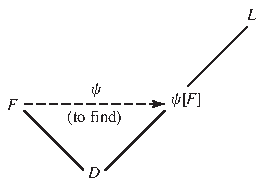
\includegraphics[width=0.359\linewidth,height=.8\textheight,keepaspectratio]{assets/p232_22.pdf}\end{center}
\begin{center}\small\textbf{26.8 Figure}\end{center}
\end{BookFloat}

\end{BookBody}

% Source PDF page 233; original printed page 216
\BookSource{233}{216}
\BookNarrativetrue

\begin{BookBody}

\noindent Every \BookInline{x\in F} is a quotient \BookInline{a/_{F}b} of some two elements \BookInline{a} and \BookInline{b,\allowbreak b\neq 0,\allowbreak } of \BookInline{D.} Let us attempt to define \BookInline{\psi } by

\begin{center}\begin{adjustbox}{max width=\linewidth}\BookInline{\displaystyle \psi (a/_{F}b)= \psi (a)/_{L}\psi (b).}\end{adjustbox}\end{center}

\noindent We must first show that this map \BookInline{\psi } is sensible and well-defined. Since \BookInline{\psi } is the identity on \BookInline{D,\allowbreak } for \BookInline{b\neq 0} we have \BookInline{\psi (b)\neq 0,\allowbreak } so our definition of \BookInline{\psi (a/_{F}b)} as \BookInline{\psi (a)/_{L}\psi (b)} makes sense. If \BookInline{a/_{F}b= c/_{F}d} in \BookInline{F,\allowbreak } then \BookInline{ad= bc} in \BookInline{D,\allowbreak } so \BookInline{\psi (ad)= \psi (bc).} But since \BookInline{\psi } is the identity on \BookInline{D,\allowbreak }

\begin{center}\begin{adjustbox}{max width=\linewidth}\BookInline{\displaystyle \psi (ad)= \psi (a)\psi (d)\;\text{and}\;\psi (bc)= \psi (b)\psi (c).}\end{adjustbox}\end{center}

\noindent Thus

\begin{center}\begin{adjustbox}{max width=\linewidth}\BookInline{\displaystyle \psi (a)/_{L}\psi (b)= \psi (c)/_{L}\psi (d)}\end{adjustbox}\end{center}

\noindent in \BookInline{L,\allowbreak } so \BookInline{\psi } is well-defined.

The equations

\begin{center}\begin{adjustbox}{max width=\linewidth}\BookInline{\displaystyle \psi (xy)= \psi (x)\psi (y)}\end{adjustbox}\end{center}

\noindent and

\begin{center}\begin{adjustbox}{max width=\linewidth}\BookInline{\displaystyle \psi (x+ y)= \psi (x)+ \psi (y)}\end{adjustbox}\end{center}

\noindent follow easily from the definition of \BookInline{\psi } on \BookInline{F} and from the fact that \BookInline{\psi } is the identity on \BookInline{D.}

If \BookInline{\psi (a/_{F}b)= \psi (c/_{F}d),\allowbreak } we have

\begin{center}\begin{adjustbox}{max width=\linewidth}\BookInline{\displaystyle \psi (a)/_{L}\psi (b)= \psi (c)/_{L}\psi (d)}\end{adjustbox}\end{center}

\noindent so

\begin{center}\begin{adjustbox}{max width=\linewidth}\BookInline{\displaystyle \psi (a)\psi (d)= \psi (b)\psi (c).}\end{adjustbox}\end{center}

\noindent Since \BookInline{\psi } is the identity on \BookInline{D,\allowbreak } we then deduce that \BookInline{ad= bc,\allowbreak } so \BookInline{a/_{F}b= c/_{F}d.} Thus \BookInline{\psi } is one-to-one.

By definition\BookInline{,\allowbreak \psi (a)= a} for \BookInline{a\in D.} \BookEnd{\blacklozenge}

\BookLabel{26.9 Corollary} Every field \BookInline{L} containing an integral domain \BookInline{D} contains a field of quotients of \BookInline{D.}

\BookLabel{\textit{Proof}} In the proof of Theorem 26.7 every element of the subfield \BookInline{\psi [F]} of \BookInline{L} is a quotient in \BookInline{L} of elements of \BookInline{D.}\BookEnd{\blacklozenge}

\BookLabel{26.10 Corollary} Any two fields of quotients of an integral domain \BookInline{D} are isomorphic.

\BookLabel{\textit{Proof}} Suppose in Theorem 26.7 that \BookInline{L} is a field of quotients of \BookInline{D,\allowbreak } so that every element \BookInline{x} of \BookInline{L} can be expressed in the form \BookInline{a/_{L}b} for \BookInline{a,\allowbreak b\in D.} Then \BookInline{L} is the field \BookInline{\psi [F]} of the proof of Theorem 26.7 and is thus isomorphic to \BookInline{F.}\BookEnd{\blacklozenge}

\end{BookBody}

\BookNarrativefalse

\begin{BookBody}

\BookExerciseTitle{26}

\BookTextHeading{\textbf{Computations}}

\BookExercise{1.}{Describe the field \BookInline{F} of quotients of the integral subdomain}

\begin{center}\begin{adjustbox}{max width=\linewidth}\BookInline{\displaystyle D= \{n+ mi\mid n,\allowbreak m\in \mathbb{Z}\}}\end{adjustbox}\end{center}

\noindent of \BookInline{\mathbb{C}.} “Describe” means give the elements of \BookInline{\mathbb{C}} that make up the field of quotients of \BookInline{D} in \BookInline{\mathbb{C}.(}The elements of \BookInline{D} are the\textbf{ Gaussian integers.})

\BookExercise{2.}{Describe (in the sense of Exercise 1) the field \BookInline{F} of quotients of the integral subdomain \BookInline{D= \{n+ m\sqrt{3}\mid n,\allowbreak m\in \mathbb{Z}\}} of \BookInline{\mathbb{R}.}}

\end{BookBody}

% Source PDF page 234; original printed page 217
\BookSource{234}{217}
\BookNarrativefalse

\begin{BookBody}

\BookTextHeading{\textbf{Concepts}}

\BookExercise{3.}{Correct the definition of the italicized term without reference to the text, if correction is needed, so that it is in a form acceptable for publication.}

A \BookInline{\text{fi}eld} \textit{of quotients} of an integral domain \BookInline{D} is a field \BookInline{F} in which \BookInline{D} can be embedded so that every nonzero element of \BookInline{D} is a unit in \BookInline{F.}

\BookExercise{4.}{Determine whether each of the following is true or false.}

\BookExercise{a.}{\textbf{a}\BookInline{.\mathbb{Q}} is a field of quotients of \BookInline{\mathbb{Z}.}}

\BookExercise{b.}{\textbf{b}\BookInline{.\mathbb{R}} is a field of quotients of \BookInline{\mathbb{Z}.}}

\BookExercise{c.}{\textbf{c}\BookInline{.\mathbb{R}} is a field of quotients of \BookInline{\mathbb{R}.}}

\BookExercise{d.}{\textbf{d}\BookInline{.\mathbb{C}} is a field of quotients of \BookInline{\mathbb{R}.}}

\BookExercise{e.}{If \BookInline{D} is a field, then any field of quotients of \BookInline{D} is isomorphic to \BookInline{D.}}

\BookExercise{f.}{The fact that \BookInline{D} has no divisors of 0 was used strongly several times in the construction of a field \BookInline{F} of quotients of the integral domain \BookInline{D.}}

\BookExercise{g.}{Every element of an integral domain \BookInline{D} is a unit in a field \BookInline{F} of quotients of \BookInline{D.}}

\BookExercise{h.}{Every nonzero element of an integral domain \BookInline{D} is a unit in a field \BookInline{F} of quotients of \BookInline{D.}}

\BookExercise{i.}{A field of quotients \BookInline{F^{\prime }} of a subdomain \BookInline{D^{\prime }} of an integral domain \BookInline{D} can be regarded as a subfield of some field of quotients of \BookInline{D.}}

\BookExercise{j.}{Every field of quotients of \BookInline{\mathbb{Z}} is isomorphic to \BookInline{\mathbb{Q}.}}

\BookExercise{5.}{Show by an example that a field \BookInline{F^{\prime }} of quotients of a proper subdomain \BookInline{D^{\prime }} of an integral domain \BookInline{D} may also be a field of quotients for \BookInline{D.}}

\BookTextHeading{\textbf{Theory}}

\BookExercise{6.}{Prove Part 2 of Step 3. You may assume any preceding part of Step 3.}

\BookExercise{7.}{Prove Part 3 of Step 3. You may assume any preceding part of Step 3.}

\BookExercise{8.}{Prove Part 4 of Step 3. You may assume any preceding part of Step 3.}

\BookExercise{9.}{Prove Part 5 of Step 3. You may assume any preceding part of Step 3.}

\BookExercise{10.}{Prove Part 6 of Step 3. You may assume any preceding part of Step 3.}

\BookExercise{11.}{Prove Part 7 of Step 3. You may assume any preceding part of Step 3.}

\BookExercise{12.}{Let \BookInline{R} be a nonzero commutative ring, and let \BookInline{T} be a nonempty subset of \BookInline{R} closed under multiplication and containing neither 0 nor divisors of 0. Starting with \BookInline{R\times T} and otherwise exactly following the construction in this section, we can show that the ring \BookInline{R} can be enlarged to a\textit{ partial ring of quotients} \BookInline{Q(R,\allowbreak T).} Think about this for 15 minutes or so; look back over the construction and see why things still work. In particular, show the following:}

\BookExercise{a.}{\textbf{a}\BookInline{.Q(R,\allowbreak T)} has unity even if \BookInline{R} does not.}

\BookExercise{b.}{In \BookInline{Q(R,\allowbreak T),\allowbreak } every nonzero element of \BookInline{T} is a unit.}

\BookExercise{13.}{Prove from Exercise 12 that every nonzero commutative ring containing an element \BookInline{a} that is not a divisor of 0 can be enlarged to a commutative ring with unity. Compare with Exercise 36 of Section 23.}

\BookExercise{14.}{With reference to Exercise 12, how many elements are there in the ring \BookInline{Q(\mathbb{Z}_{4},\allowbreak \{1,\allowbreak 3\})}?}

\BookExercise{15.}{With reference to Exercise 12, describe the ring \BookInline{Q(\mathbb{Z},\allowbreak \{2^{n}\mid n\in \mathbb{Z}^{+ }\}),\allowbreak } by describing a subring of \BookInline{\mathbb{R}} to which it is isomorphic.}

\BookExercise{16.}{With reference to Exercise 12, describe the ring \BookInline{Q(3\mathbb{Z},\allowbreak \{6^{n}\mid n\in \mathbb{Z}^{+ }\})} by describing a subring of \BookInline{\mathbb{R}} to which it is isomorphic.}

\BookExercise{17.}{With reference to Exercise 12, suppose we drop the condition that \BookInline{T} have no divisors of zero and just require that nonempty \BookInline{T} not containing 0 be closed under multiplication. The attempt to enlarge \BookInline{R} to a commutative ring with unity in which every nonzero element of \BookInline{T} is a unit must fail if \BookInline{T} contains an element \BookInline{a} that is a divisor of 0, for a divisor of 0 cannot also be a unit. Try to discover where a construction parallel to that in the text but starting with \BookInline{R\times T} first runs into trouble. In particular, for \BookInline{R= \mathbb{Z}_{6}} and \BookInline{T= \{1,\allowbreak 2,\allowbreak 4\},\allowbreak } illustrate the first difficulty encountered. [\textit{Hint:} It is in Step 1.]}

\end{BookBody}
\ifdefined\BookMaster\let\BookFinish\relax\else\def\BookFinish{\end{document}}\fi\BookFinish
